%%%%%%%%%%%%%%%%%%%%%%%%%%%%%%%%%%%%%%%%%
% Beamer Presentation
% LaTeX Template
% Version 1.0 (10/11/12)
%
% This template has been downloaded from:
% http://www.LaTeXTemplates.com
%
% License:
% CC BY-NC-SA 3.0 (http://creativecommons.org/licenses/by-nc-sa/3.0/)
%
%%%%%%%%%%%%%%%%%%%%%%%%%%%%%%%%%%%%%%%%%

%----------------------------------------------------------------------------------------
%	PACKAGES AND THEMES
%----------------------------------------------------------------------------------------

\documentclass{beamer}
\usepackage{eucal}
\usepackage{lmodern}
\usepackage{color, colortbl, linegoal}
\usepackage{setspace}
\usepackage{svg}
\usepackage{pgfplots}

\mode<presentation> {

% The Beamer class comes with a number of default slide themes
% which change the colors and layouts of slides. Below this is a list
% of all the themes, uncomment each in turn to see what they look like.

%\usetheme{default}
%\usetheme{AnnArbor}
%\usetheme{Antibes}
%\usetheme{Bergen}
%\usetheme{Berkeley}
%\usetheme{Berlin}
%\usetheme{Boadilla}
%\usetheme{CambridgeUS}
%\usetheme{Copenhagen}
%\usetheme{Darmstadt}
%\usetheme{Dresden}
%\usetheme{Frankfurt}
%\usetheme{Goettingen}
%\usetheme{Hannover}
%\usetheme{Ilmenau}
%\usetheme{JuanLesPins}
%\usetheme{Luebeck}
\usetheme{Madrid}
%\usetheme{Malmoe}
%\usetheme{Marburg}
%\usetheme{Montpellier}
%\usetheme{PaloAlto}
%\usetheme{Pittsburgh}
%\usetheme{Rochester}
%\usetheme{Singapore}
%\usetheme{Szeged}
%\usetheme{Warsaw}

% As well as themes, the Beamer class has a number of color themes
% for any slide theme. Uncomment each of these in turn to see how it
% changes the colors of your current slide theme.

%\usecolortheme{albatross}
%\usecolortheme{beaver}
%\usecolortheme{beetle}
%\usecolortheme{crane}
%\usecolortheme{dolphin}
%\usecolortheme{dove}
%\usecolortheme{fly}
%\usecolortheme{lily}
%\usecolortheme{orchid}
%\usecolortheme{rose}
%\usecolortheme{seagull}
%\usecolortheme{seahorse}
%\usecolortheme{whale}
%\usecolortheme{wolverine}

%\setbeamertemplate{footline} % To remove the footer line in all slides uncomment this line
%\setbeamertemplate{footline}[page number] % To replace the footer line in all slides with a simple slide count uncomment this line

%\setbeamertemplate{navigation symbols}{} % To remove the navigation symbols from the bottom of all slides uncomment this line
}

\usepackage{graphicx} % Allows including images
\usepackage{booktabs} % Allows the use of \toprule, \midrule and \bottomrule in tables


\usepackage{hyperref}
\hypersetup{
    colorlinks=true,
    linkcolor=blue,
    filecolor=magenta,      
    urlcolor=cyan,
}

\urlstyle{same}

\usepackage[utf8]{inputenc}
\usepackage{tikz}
\usetikzlibrary{calc,math}
\usepackage{amsmath}
\DeclareMathOperator*{\argmax}{arg\,max}
\DeclareMathOperator*{\argmin}{arg\,min}
\newcommand{\true}{\texttt{true}}
\newcommand{\false}{\texttt{false}}

%----------------------------------------------------------------------------------------
%	TITLE PAGE
%----------------------------------------------------------------------------------------

\title[Segment Set Cover]{Approximation and parameterization\\
of Segment Set Cover}
% The short title appears at the bottom of every slide, the full title is only on the title page

\author{Katarzyna Kowalska, Michał Pilipczuk} % Your name
\institute[UW] % Your institution as it will appear on the bottom of every slide, may be shorthand to save space
{
University of Warsaw, MIMUW \\ % Your institution for the title page
\medskip
\textit{kk371053@students.mimuw.edu.pl} % Your email address
}
\date{21.06.2022} % Date, can be changed to a custom date

\begin{document}

\begin{frame}
\titlepage % Print the title page as the first slide
\end{frame}

\begin{frame}
\frametitle{Overview} % Table of contents slide, comment this block out to remove it
\tableofcontents % Throughout your presentation, if you choose to use \section{} and \subsection{} commands, these will automatically be printed on this slide as an overview of your presentation
\end{frame}

\definecolor{olivegreen}{HTML}{2a9d8f}
\definecolor{shary}{HTML}{8d99ae}

%----------------------------------------------------------------------------------------
%	PRESENTATION SLIDES
%----------------------------------------------------------------------------------------

\section{\textsc{Set Cover}}
\begin{frame}
\frametitle{Problem Statement: \textsc{Set Cover}}
\textbf{Input:} universe $\mathcal{U}$,
family $S$ of subsets of $\mathcal{U}$
\newline
\textbf{Output:} $C \subseteq S$ such that $|C|$ is minimal and
$\bigcup C = \mathcal{U}$
\newline
Minimal subfamily that covers all elements in $\mathcal{U}$.

\begin{center}
\includesvg[width=0.5\textwidth]{figures/set_cover.svg}
\end{center}

\end{frame}
\subsection{\textsc{Geometric Set Cover}}

\begin{frame}
\frametitle{Problem Statement: \textsc{Geometric Set Cover}}
\begin{itemize}
\item Universe $\mathcal{U}$ is set of points in the plane
\item Sets $S$ are some geometric shapes
\item Formally, each set in $S$ is intersection of $\mathcal{U}$
with some geometric shape.
\end{itemize}

Example for rectangles:

\includesvg[width=0.5\textwidth]{geometric_set_cover.svg}


\end{frame}
\subsection{\textsc{Segment Set Cover}}

\begin{frame}
\frametitle{Problem Statement: \textsc{Segment Set Cover}}
\begin{itemize}
\item Universe $\mathcal{U}$ is a set of points in the plane.
\item Sets $S$ are line segments.
\end{itemize}

\begin{center}
\includesvg[width=0.5\textwidth]{figures/segment_cover.svg}
\end{center}


\end{frame}

\section{$\delta$-extension}
\begin{frame}
\frametitle{$\delta$-extension for \textsc{Segment Set Cover}}
\begin{itemize}
\item $\delta$-extension for a segment is a segment which is longer by
$\delta$ fraction at both ends
\item We accept solution in which segments cover solution after
$\delta$-extension
\item The solution is compared to optimal solution without extension.
\end{itemize}

Example:

\includesvg[width=0.35\textwidth]{delta_extension.svg}

It is based on similar concept of $\delta$-shrinking,
which helped to provide FPT algorithm and EPTAS for 
(originally W[1]-hard and APX-hard)
\textsc{Maximum Weight Independent Set of Rectangles}.
\end{frame}

\section{Approximation}
\begin{frame}
\frametitle{Preliminaries: Approximation}
Given:
\begin{itemize}
\item instance $I$ of the optimization problem (looking for minimal solution)
\item weight of the optimal solution $\mathsf{opt}(I)$
\end{itemize}
$p$-approximation is algorithm that yields solution of weight not larger than
$p\cdot \mathsf{opt}(I)$
\begin{block}{PTAS -- polynomial time approximation scheme}
For every $\epsilon > 0$, there exists $(1+\epsilon)$-approximation
algorithm running in time $n^{f(\epsilon)}$ for some computable function $f$.

Example: \textsc{Knapsack}.

\end{block}

\begin{block}{APX-hardness}
For sufficiently small $\epsilon > 0$,
if $(1+\epsilon)$-approximation exists, then P = NP.

Example: \textsc{MAX-3-SAT} (how many clauses in 3-SAT can be solved)
\end{block}


\end{frame}
\begin{frame}
\frametitle{Approximation results for \textsc{Set Cover} from literature}
\textsc{Set Cover}
\begin{itemize}
\item $\log n$ approximation, no $o(\log n)$ approximation assuming P $\neq$ NP
\end{itemize}

\textsc{Geometric Set Cover}
\begin{itemize}
\item with fat rectangles is APX-hard
\item EPTAS for fat polygons with $\delta$-extension \textbf{[Har-Peled and Lee, 2012]}
\end{itemize}


\begin{definition}{
Fatness of polygons $\tau$ is a ratio between a radius of circle
circumscribed on this polygon and inscribed in this polygon.
}\end{definition}
\includesvg[width=0.2\textwidth]{fat_polygon.svg}

\end{frame}

\begin{frame}{\textsc{MAX-(3,3)-SAT}}
How do we prove that there doesn't exist $(1+\epsilon)$-approximation?


\begin{block}{\textsc{MAX-(3,3)-SAT} problem}
Given 3-SAT instance with $n$ variables, $m$ clauses
and every variable appears in exactly 3 clauses,
find an assignment
that satisfies the maximum number of clauses
(not necessarily all of them).
\end{block}

MAX-(3,3)-SAT is NP-complete, therefore:

\begin{block}{NP-completeness}
Distinguishing if result of MAX-(3,3)-SAT is
$n$ or less than $n$ is NP-complete.
\end{block}
\end{frame}

\begin{frame}{PCP theorem}
\begin{block}{PCP Theorem}
NP = PCP($\log n$, $\mathcal{O}(1)$).
\end{block}

\begin{block}{PCP theorem implication [Håstad, 2001]}
Distinguishing whether optimum result of
the instance of MAX-(3,3)-SAT is $m$
or at most $\frac{49}{50} \cdot m$ is NP-hard.
\end{block}

Therefore MAX-(3,3)-SAT does not have
$(1+\frac{1}{49})$-approximation
\end{frame}


\begin{frame}
\frametitle{Approximation of \textsc{Segment Set Cover}}
\begin{block}{Theorem 1}
	\textsc{Segment Set Cover} is APX-hard, i.e.
	there exists such $\epsilon>0$
	that $(1+\epsilon)$-approximation 
	running in time $n^{f(\epsilon)}$ does not exist if P $\neq$ NP.
\end{block}

How can we make this problem \textit{easier}?
\begin{itemize}
\item Allow only segments in 2 directions (parallel to the two axes)
\item Allow segments to \textit{almost} cover the points, i.e. $\delta$-extension
\end{itemize}

\pause

\bigskip

\textbf{Remark:}
	Set cover with polygons of bounded fatness (at least $\tau$):
	\begin{enumerate}
	\item is APX-hard;
	\item with $\delta$-extension has EPTAS.
	\end{enumerate}

\end{frame}

\begin{frame}
\begin{block}{Theorem 1 (rephrased)}
	\textsc{Segment Set Cover} is APX-hard, even if segments are axis-parallel
	and problem is relaxed with $\frac{1}{2}$-extension.
\end{block}

\begin{figure}
\centering
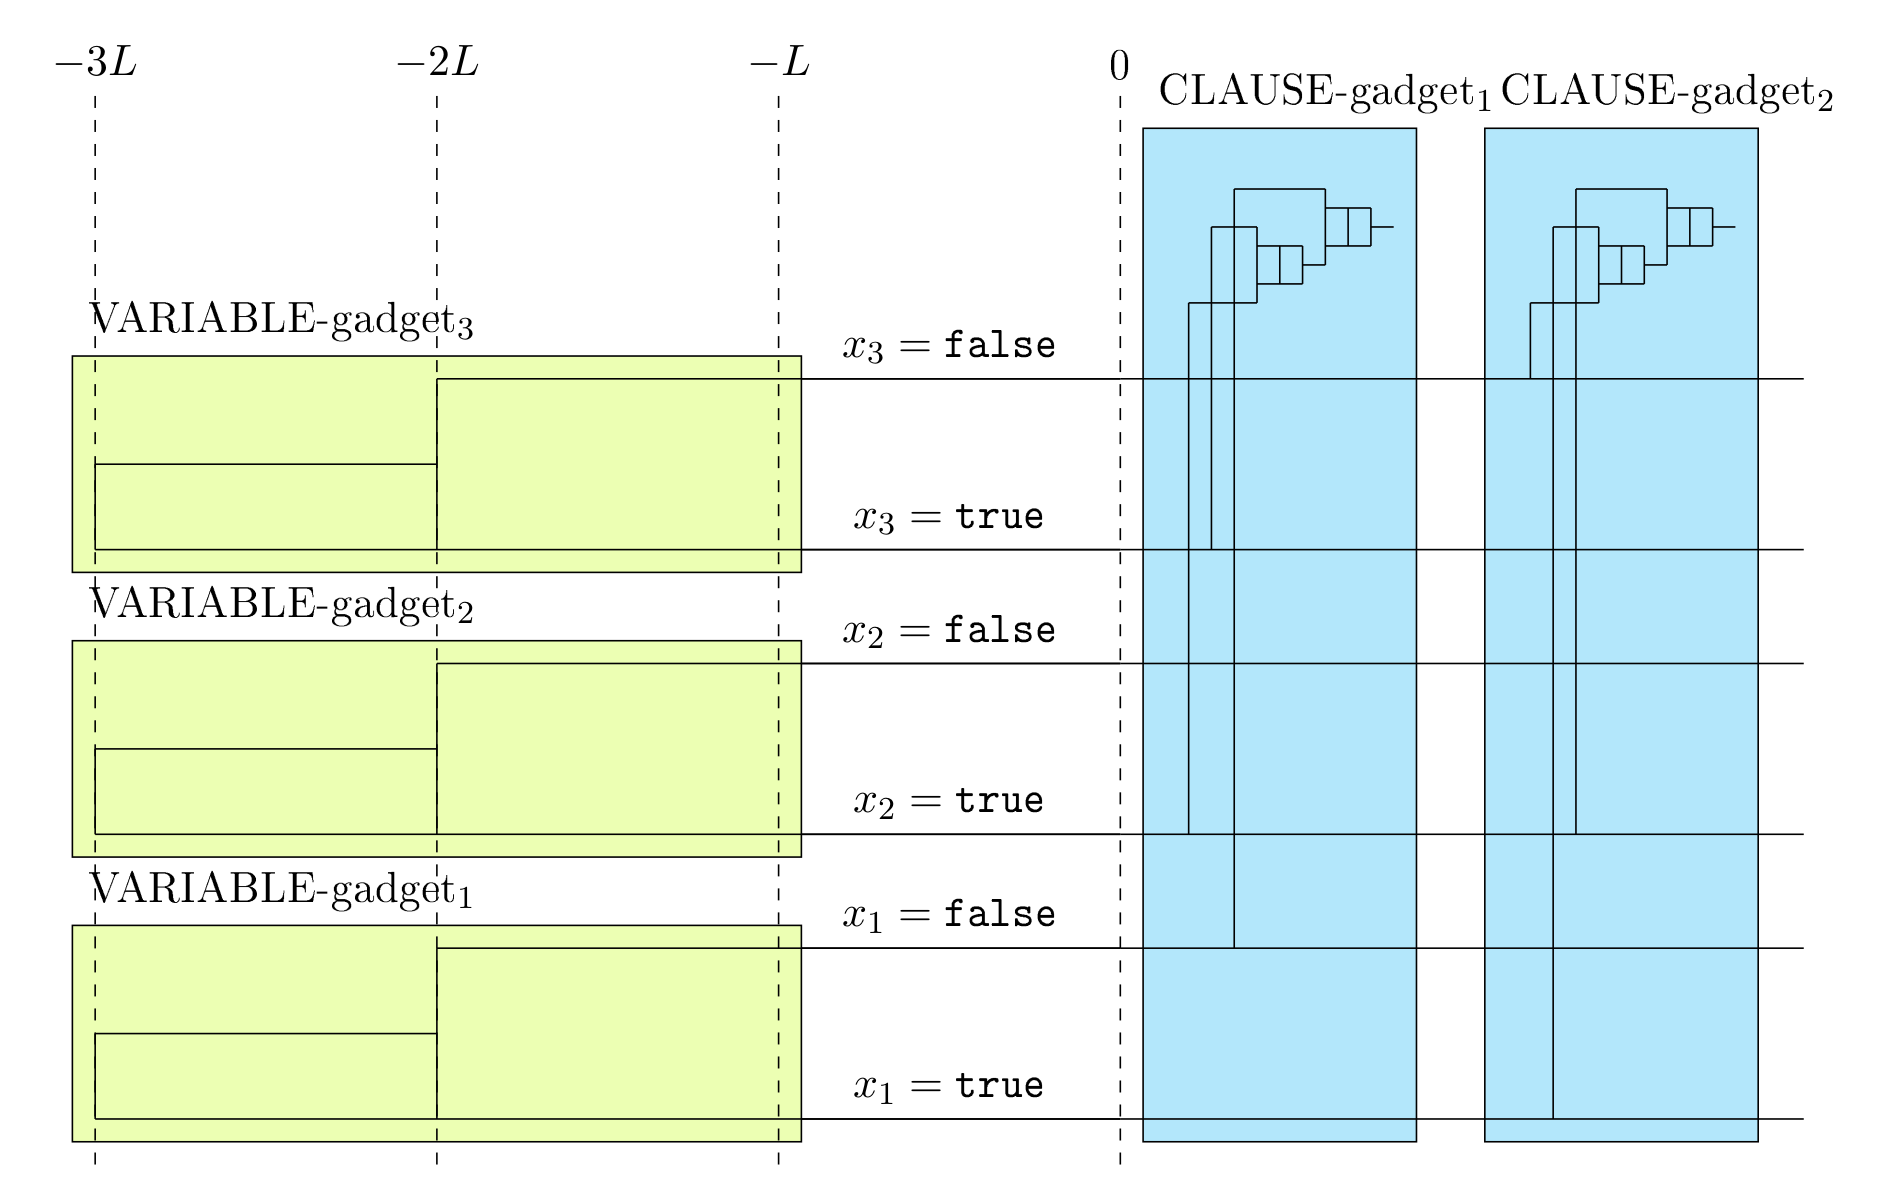
\includegraphics[scale=0.1]{figures/apxhard.png}
\caption{Scheme of the construction.}
\end{figure}

\end{frame}


\begin{frame}
\frametitle{Results for approximation of \textsc{Geometric Set Cover}}
\begin{tabular}{|c|c|c|}
\hline
           & exact & $\delta$-extension \\
\hline
fat polygons & APX-hard  &  EPTAS \\
& [Chan and Grant, 2014] & [Har-Peled and Lee, 2012] \\
\hline
segments & \textcolor{olivegreen}{APX-hard*} & \textcolor{olivegreen}{APX-hard (Theorem 1)} \\
\hline
any polygons & APX-hard* &  \textcolor{olivegreen}{APX-hard*} \\
\hline
\end{tabular}

\bigskip
Results marked with * follow from results for more restricted settings.

\end{frame}

\section{Parameterization}

\begin{frame}
\frametitle{Prelimiaries: Parameterized algorithms}
Instance $I$ of a parameterized problem now has:
\begin{itemize}
\item size of the instance $n$;
\item parameter $k$ (usually size of the solution).
\end{itemize}
\bigskip

\begin{tabular}{|c|c|c|}
\hline
\textbf{Class} & \textbf{Upper Bound of Complexity} & \textbf{Example}\\
\hline
FPT & $f(k) \cdot n^{O(1)}$ & \textsc{Vertex Cover}\\
\hline
W[1] & $n^{O(k)}$ & \textsc{$k$-Clique}, \textsc{Grid Tiling}\\
\hline
\end{tabular}

\pause

\bigskip
\textsc{Set Cover} is:
\begin{itemize}
\item W[2]-complete
\item no algorithm with running time $n^{k-\epsilon}$ for any $\epsilon > 0$
\end{itemize}
\end{frame}

\begin{frame}
\frametitle{Parameterization of \textsc{Geometric Set Cover}}
\begin{block}{Theorem [Marx, 2005]}
	\textsc{Geometric Set Cover} 
	with unit squares parameterized by the solution size $k$
	is W[1]-hard.
\end{block}

The follow-up work [Marx and Pilipczuk, 2022]
shows a tight bound for this problem $n^{\mathcal{O}(\sqrt{k})}$.

\end{frame}

\begin{frame}
\frametitle{Parameterization of \textsc{Segment Set Cover}}
\begin{block}{Theorem 2}
	\textsc{Segment Set Cover} parameterized by the solution size $k$
	can be solved in time $k^k \cdot n^{O(1)}$.
\end{block}

\textbf{Technique:} Branching over at most $k+1$
segments on the lines with more than $k$ points on them.

\pause

\bigskip

Now let's make problem \textcolor{red}{\textbf{harder}}...

\end{frame}

\section{\textsc{Weighted Segment Set Cover}} 

\begin{frame}
\frametitle{Definition of \textsc{Weighted Segment Set Cover}}

\textbf{Input:} universe $\mathcal{U}$,
subfamily $S$ of subsets of $\mathcal{U}$
and function of weights assigned to sets $w : S \rightarrow \mathbb{R^+}$
\newline
\textbf{Output:} $C \subseteq S$ such that $\sum_{c \in C} w(c)$ is minimal and
$\bigcup C = \mathcal{U}$
\newline
Minimal subfamily that covers all elements in $\mathcal{U}$.

\pause

\bigskip
\textbf{In parameterized setting:}
We look for the \textit{best} solution with restricted size $|C| \le k$.

\textbf{In approximation setting:}
It is still APX-hard, nothing interesting
\bigskip
\pause

\textbf{FPT results for weighted problems in literature:}
\begin{itemize}
\item general weighted FPT framework {[Shachnai and Zehavi, 2017]}
\item kernels for \textsc{Weighted Subset Sum}, \textsc{Weighted Knapsack} {[Etscheid et al.,2017]}
\item \textsc{Weighted $st$-Cut} \textsc{Weighted Directed Feedback Set} {[Kim et al., 2021]}
\end{itemize}


\end{frame}

\begin{frame}
\frametitle{Parameterization of \textsc{Weighted Segment Set Cover}}
\begin{block}{Theorem 3}
	\textsc{Weighted Segment Set Cover} is W[1]-hard
	and there does not exists an algorithm running in time $n^{o(\sqrt{k})}$.
\end{block}


This result is particularly interesting, because unweighted problem 
has an FPT algorithm.

\bigskip

How can we make this problem easier?
\begin{itemize}
\item allow less directions (maybe just two parallel to axes);
\item allow $\delta$-extension.
\end{itemize}
\end{frame}

\begin{frame}
\frametitle{Parameterization of \textsc{Weighted Segment Set cover}}

\begin{block}{Theorem 3 (rephrased)}
	\textsc{Weighted Segment Set cover} is W[1]-hard
	and there does not exists an algorithm running in time $n^{o(\sqrt{k})}$
	even when segments are limited to 3 directions.
\end{block}

\end{frame}

\begin{frame}
\frametitle{Parameterization of \textsc{Weighted Segment Set Cover}}
\begin{block}{Theorem 4}
	\textsc{Weighted Segment Set Cover} relaxed
	with $\delta$-extension has an FPT algorithm.
	
	It can be solved with algorithm running in time $\mathcal{O}((2+k/\delta)^k \cdot n^{O(1)})$.
\end{block}

\textbf{Technique intuition:} Provide a kernel where we choose
\textbf{$(k, \delta)$-good} set of points of size at most $f(k, \delta)$
on each line with more than $k+1$ points on them.

Subset of a set of collinear points $S$
is \textbf{$(k, \delta)$-good}
if no matter how we cover it with $k$
segments, then these segments after $\delta$-extension
cover all points from the original set of points $S$.
\end{frame}

\begin{frame}
\frametitle{Results of parameterization of \textsc{Geomtric Set Cover}}


\textsc{Geometric Set Cover}
\begin{tabular}{|c|c|c|}
\hline
           & exact & $\delta$-extension \\
\hline
fat polygons & W[1]-hard [Marx, 2005] & ??? \\
\hline
segments &  \textcolor{olivegreen}{FPT (Theorem 2)} & \textcolor{olivegreen}{FPT*} \\
\hline
\end{tabular}

\bigskip

\textsc{Segment Set Cover}
\begin{tabular}{|c|c|c|}
\hline
           & exact & $\delta$-extension \\
\hline
unweighted & \textcolor{olivegreen}{FPT (Theorem 2)} & \textcolor{olivegreen}{FPT*} \\
\hline
weighted 2 directions & ??? & \textcolor{olivegreen}{FPT*} \\
\hline
weighted 3 directions & \textcolor{olivegreen}{W[1]-hard (Theorem 3)} &  \textcolor{olivegreen}{FPT*}\\
\hline
weighted any directions & \textcolor{olivegreen}{W[1]-hard*} &  \textcolor{olivegreen}{FPT (Theorem 4)}\\
\hline
\end{tabular}

\end{frame}


\begin{frame}
\begin{block}{Theorem 3 (reminder)}
	\textsc{Weighted Segment Set cover} is W[1]-hard
	and there does not exists an algorithm running in time $n^{o(\sqrt{k})}$
	even when segments are limited to 3 directions.
\end{block}
\bigskip

\textbf{Future work:}
\begin{itemize}
\item prove Theorem 3 for axis-parallel segments (2 directions);
\item remove the gap between the lower bound of complexity $n^{o(\sqrt{k})}$
and a simple algorithm running in time $n^{\mathcal{O}(k)}$;
\item investigate whether $\textsc{Geometric Set Cover}$ 
with fat polygons relaxed with $\delta$-extension has FPT algorithm.
\end{itemize}
\end{frame}

\begin{frame}
\begin{center}
The end.
\end{center}
\end{frame}

%----------------------------------------------------------------------------------------

\end{document} 
